\textbf{Алгоритм Грехема.} 
\begin{enumerate}
    \item Пусть $P_0$ — самая нижняя (из них самая левая) точка.
    \item Отсортируем точки относительно угла между $OX$ и $P_0P_i$ (при равенстве по |$P_0P_i$|).
    \item Добавим в стек $S$ точки $P_0, P_1$.
    \item Если угол поворота(против часовой стрелки) от $S.prevtop() S.top()$ до $S.top()P_i$ меньше $\pi$, добавляем $P_i$ в стек. Иначе, пока угол больше $\pi$, извлекаем из стека последнюю точку.
\end{enumerate}
В конце алгоритма в стеке будет лежать выпуклая оболочка.\newline

%\begin{figure}[h]
%    \centering
%    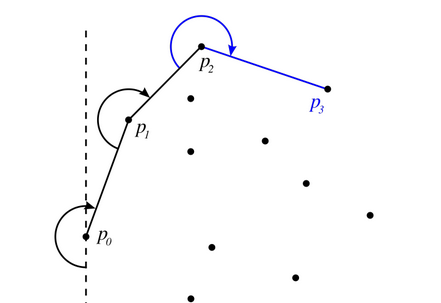
\includegraphics[scale = 0.8]{pix/convex_hull_Jarvis.png}
%\end{figure}

\textbf{Aсимптотика:} Первые две стадии: поиск $P_0$ и сортировка работают за $O(n\cdot\log n)$
времени. За сколько работает проход стеком? За линейное время, так как каждая точка попадает в стек ровно раз и не более одного раза оттуда удаляется.

Таким образом, суммарное время работы составит $O(n\cdot\log n)$.\newline

Псевдокод:
\begin{lstlisting}
p0 = TheLeftestAmongTheLowests(points);
sort(points, by_polar_from(p0));
stack<point> s;
s.push(points[0]), s.push(points[1]);
for (int i = 2; i < points.size(); ++i) {
  while (s.size() >= 2 &&
      Angle(s.prevtop(), s.top(), points[i]) < pi) {
        s.pop();
  }
  s.push(points[i]);
}
\end{lstlisting}
\pagebreak